%  $Description: Author guidelines and sample document in LaTeX 2.09$
%
%  $Author: ienne $
%  $Date: 1995/09/15 15:20:59 $
%  $Revision: 1.4 $
%
%\documentclass[times, 10pt,twocolumn]{article}
\documentclass[conference,final]{IEEEtran}
\usepackage{latex8}
\usepackage{times}

% Users' option
\usepackage{amssymb}
\usepackage{amsmath}
\usepackage{graphicx}
\usepackage{epstopdf}
\usepackage{color}
\topmargin=0.01in
\usepackage{multirow}
\usepackage{booktabs}
\newif\ifdraft
\drafttrue

\renewcommand{\multirowsetup}{\centering}
\renewcommand{\arraystretch}{1.2}
\def\nyc{\centering}

\ifdraft
\newcommand{\fixme}[1]{ { \bf{ ***FIXME: #1 }} }
\newcommand{\jhanote}[1]{ {\textcolor{red} { ***Jha: #1 }}}
\newcommand{\Nkimnote}[1]{ {\textcolor{green} { ***Nkim: #1 }}}
\newcommand{\skonote}[1]{ {\textcolor{blue} { ***Jeff: #1 }}}
\newcommand{\athotanote}[1]{ {\textcolor{green} { ***athota: #1 }}}
\newcommand{\Jkimnote}[1]{ {\textcolor{red} { ***Jkim: #1 }}}
\newcommand{\yyenote}[1]{ {\textcolor{blue} { ***yye00: #1 }}}
\else
\newcommand{\jhanote}[1]{}
\newcommand{\Nkimnote}[1]{}
\newcommand{\fixme}[1]{}
\newcommand{\skonote}[1]{}
\newcommand{\Jkimnote}[1]{}
\fi
% End of users' option

%\documentstyle[times,art10,twocolumn,latex8]{article}

%-------------------------------------------------------------------------
% take the % away on next line to produce the final camera-ready version
\pagestyle{empty}

\newcommand{\up}{\vspace*{-1em}}
\newcommand{\upp}{\vspace*{-0.5em}}
\newcommand{\ts}{$T_{s}$}


%-------------------------------------------------------------------------
\title{Efficient Runtime Environment for Coupled Multi-Physics Simulations: \\
Dynamic Resource Allocation and Load-Balancing}

% \author{Soon-Heum Ko, Nayong Kim, Joohyun Kim, Abhinav Thota, Shantenu Jha\\
% Center for Computation and Technology\\
% Louisiana State University, Baton Rouge, LA 70803, USA\\
% (sko,nykim,jhkim,athota1,sjha)@cct.lsu.edu\\
% % For a paper whose authors are all at the same institution,
% % omit the following lines up until the closing ``}''.
% % Additional authors and addresses can be added with ``\and'',
% % just like the second author.
% %\and
% % Dimitris Nikitopoulos\\
% % Mechanical Engineering Department\\
% % Louisiana State University, Baton Rouge, LA 70803, USA\\
% % meniki@lsu.edu\\
% \and
% Yaakoub El Khamra\\
% Texas Advanced Computing Center\\
% The University of Texas at Austin, Austin, Texas 78758, USA\\
% yye00@austin.mail.address\\
% }

\author{
 ~\\[-2em]
 Soon-Heum Ko$^{1}$, Nayong Kim$^{1}$, Joohyun Kim$^{1}$, \\ Abhinav Thota$^{1}$, Shantenu Jha$^{*1,2}$\\
 \small{\emph{$^{1}$Center for Computation \& Technology, Louisiana State University, USA}}\\
 \small{\emph{$^{2}$Department of Computer Science, Louisiana State University, USA}}\\
 \small{\emph{$^{*}$Contact Author}}\\
}

%\thispagestyle{empty}

\begin{document}

\maketitle

\begin{abstract}
  Coupled Multi-Physics simulations, such as hybrid CFD-MD
  simulations, represent an increasingly important class of scientific
  applications.  Often the physical problems of interest demand the
  use of high-end computers, such as TeraGrid resources, which are
  often accessible only via batch-queues. Batch-queue systems are not
  natively developed to support the coordinated scheduling of jobs --
  which in turn is required to support the concurrent execution
  required by coupled multi-physics simulations. In this paper we
  develop and demonstrate a novel approach to overcome the lack of
  native support for coordinated job submission requirement associated
  with coupled runs. Our solution is a generalization of the Pilot-Job
  concept -- which in of itself is not new, but is applied to coupled
  simulations for the first time. Our solution not only overcomes the
  initial co-scheduling problem, but provides a dynamic resource
  allocation mechanism. Support for such dynamic resources is critical
  for a load-balancing mechanism, which we develop and demonstrate to
  be effective at reducing the total time-to-solution of the
  problem. We establish that the performance advantage of using
  bigjobs is invariant with the size of the machine as well as the
  size of the physical model under investigation.  The Pilot-Job
  abstraction is developed using SAGA (http://saga.cct.lsu.edu), which
  provides an infrastructure agnostic implementation, and which can
  seamlessly execute and utilize distributed resources. We also
  demonstrate for the first time that we are aware of, the use of
  multiple Pilot-Job implementations to solve the same problem;
  specifically, we use SAGA to access the SAGA-based Pilot-Job on
  high-end resources such as the TeraGrid, whilst using the native
  Condor Pilot-Job (Glide-in) on Condor resources. Importantly both
  are invoked via the same interface without changes at the
  development or deployment level, but only an execution (run-time)
  decision.
\end{abstract}
\up\up

\jhanote{Notes: (i) We have established that the performance advantage
  of using bigjobs is invariant with the size of the machine, i.e.,
  small LONI machines such as Eric, to the largest machines available
  such as Ranger. This is not so much about the machine, but the
  system sizes of the physical-models that we are investigating. (ii)
  Need to establish clearly how we are measuring the times in Table
  I. Are we using 'startq'? Remember enough details should be
  presented to make the experiments reproducible (iii) What is the
  largest system size that we can simulate using BigJob and/or using
  independent execution threads? (iv) What is the final ratio of
  $N_{MD} to N_{CFD}$? Is it always the same? How do we counter the
  argument that the final configuration can be determined with a few
  simple pre-processing runs? What is the importance of dynamic
  resource management, i.e. start with initial Configuration I and
  adapt to Final Configuration F with intermediate states in between?
}


%-------------------------------------------------------------------------
\section{Introduction}

Coupled Multi-Physics simulation techniques are being increasingly
used to study many different physical phenomenon spanning time and
length scales at different level of
details~\cite{Tai}~\cite{Watanabe}. These techniques have been used to
investigate phenomena from crack-propagation in materials, biological
systems as well as understanding multi-phase fluid flow in constrained
geometry.

In addition to the ``physics challenges'' of these Multi-Physics
coupled simulations, there exist interesting ``computational
challenges''. Probably the best known (and investigated) is the
challenge of simulating large and complex systems, leading to
simulations that require greater computational resources -- often
involving HPC resources. % and no longer working on dedicated PCs.
Parallelization helps individual codes address the computational
demand of large and complex systems, but incorporating two distinct
codes under the umbrella of a single tightly-coupled application (say
using MPI) is not without significant problems. For example, the two
codes can often have very different computational kernels (one could
be mesh-based, the other unstructured particle simulations) with very
different computational time-scales.

Here we will focus on the challenges arising from running
tightly-coupled simulations on production systems with batch-queues,
whereby it cannot be guaranteed that two separate jobs will execute
concurrently. Specifically we will consider the case of coupling a
Computational Fluid Dynamics (CFD) code and a Molecular Dynamics (MD)
code, where the communication is via the exchange of files and not
Unix pipes (see next section for details on the coupling).

% Users' account loss is inevitable in conventional queuing systems
% except when sufficient CPUs are idling,

Although not exactly tightly-coupled in the sense of MPI, viz., very
frequent and with an extreme sensitivity to latency in communication
delay, the CFD and MD codes communicate frequently, (e.g., the CFD
code conducts data exchange in every iteration) and thus they need to
run concurrently. Thus, without explicit support for co-scheduling, it
is unlikely that coupled CFD-MD simulations will run concurrently as
inevitably the first job to run will have to wait for the other to
follow.

% \jhanote{Place the following appropriately} Thus, the best way using
% conventional job submission system would be to find a site with
% sufficient resource pool and submit two jobs with the optimal number
% of processors according to the pre-test data on performance of each
% tool in that facility with the same problem size.

Another important challenge, especially for large-scale simulations is
the need for efficient load-balancing, taking into account the
individual simulation performance. Even if the two simulations could
run concurrently, without explicit load-management/balancing support,
there is likely to be inefficient utilization of compute resources due
to load imbalance. As the performance of each simulation component
changes with computing resource and problem size, re-adjustment of
allocated resources to each task according to their performance is
required during the simulation. Interestingly, as we will show,
effective load-balancing of two independent but concurrently running
codes introduces the need for dynamic resource allocation, and the
same solution that we devise to overcome the concurrent scheduling
requirement/constraints of coupled jobs also supports the feature of
dynamic resource allocation. In contrast, if simulations were
submitted as independent jobs, changing resource (CPU) allocation to
address these changes is challenging -- as the change in resource
assigned to one is correlated with a change in resource assigned to
the other component.

The pilot-job is just a container task where a number of sub-tasks can
run in pre-defined schedule with the specified number of processors
whether or not they are coupled.  The dynamical resource allocation
capabilties of the Pilot-Job prove useful in the other two scenarios,
as well as when using load-balancing in the single-resource scenario.
Although the container-Job/Pilot-Job concept is not novel {\it per
  se}, we believe this is the first documented utilization of these
abstractions to perform coupled Multi-Physics simulations. We claim
that there several distinct advantages that arise as a consequence of
using Pilot-Jobs for Coupled Simulations: (i) obviates the need for a
o-scheduler while preserving performance, (ii) enables dynamic
resource allocation, which in turn is important for load-balancing
across coupled simulations.  But given the lack of system or
service-level support to address the challenges outlined above, there
is a need to address the solution at the application level. This paper
aims to provide novel solutions to the above problem using frameworks
that are in user (application) space.
 
We will provide details on how we implement our solution in Section 3,
but in a nutshell it is critical to mention that our solution and its
concomittant efficiency is not tied to either a specific application
set (or infrastructure) and is scalable and extensible. It is based
upon the SAGA (the Simple API for Grid Applications)~\cite{saga_web},
which is a high-level API which provides the basic functionality
required to implement distributed functionally -- both logically and
physically, in an infrastructure and middleware independent
fashion. SAGA enables the creation of higher-levels of abstractions,
for example a container-job and pilot-job (which as we will discuss is
referred to as the BigJob~\cite{saga_royalsoc}). The SAGA-based
Pilot-Job is infrastructure neutral, unlike {\it all} other
Pilot-Jobs.

We begin the next section with an outline of the basic motivation for
coupled simulations and load balancing.  We will address the
fundamental question: Does the use of an infrastructure independent
container job assist in the time to solution of coupled simulation? We
will determine that the answer is yes for a variety of different
resource utilization scenarios. In the simplest case of a coupled
simulation running on a single machine, we will establish that the
reason is the lowered waiting time typically associated with a larger
size request (on most queuing systems, for most commonly occuring load
factors).  As our experiments will show, performance improvement arise
from removing the need for scheduling the two-components separately
and in providing a single job-requirement to the queuing system.

\jhanote{Next few paragraphs need attention}

\skonote{Please leave unchanged on this section now:I'll take a look at that after changing section 5-B and 5-C}
% -------------------------------------------------------------------------
\section{Hybrid CFD-MD Approach: Understanding the Coupling,
  Communication and Load-Balancing Requirements}

The hybrid CFD/MD approach~\cite{Thompson},~\cite{Nie},~\cite{Yen} is
a simulation method which adopts the continuum hypothesis in capturing
macroscopic features of a flow-field and details atomistic
intermolecular interactions on interfaces of different materials by
using the MD approach. CFD can accurately predict flow properties on
conventional moderate/large size fluid domains, but is intrinsically
impossible to reflect characteristics of surrounding solid materials.
While MD can provide atomistic level resolution of interactions
between particles, it becomes computationally demanding as the size of
simulated system grows. The hybrid approach provides a good balance
between computational cost and atomistic details/resolution.

% when reduction of total computational cost and keeping the atomistic
% details are equivalently demanded.

A scientific problem that can be effectively tackled by the hybrid
CFD/MD approach would be, for example, the simulation of a flow-field
where the viscous effect of solid boundary is so dominant that the
length scale required becomes significantly larger than the typical
size of a system conducted by the conventional MD. Additionally,
understanding of this fluid system near the wall is profoundly
important but can be achieved only through atomistic molecular
dynamics. One solution is, as is seen in Fig.~\ref{Fig:Couette}, to
carry out the hybrid CFD/MD approaches with which atomistic
interactions between solid elements and fluid particles near the wall
is simulated by MD and the far field flow is calculated by CFD.

%%%%% FIGURE %%%%%
\begin{figure}
\centering
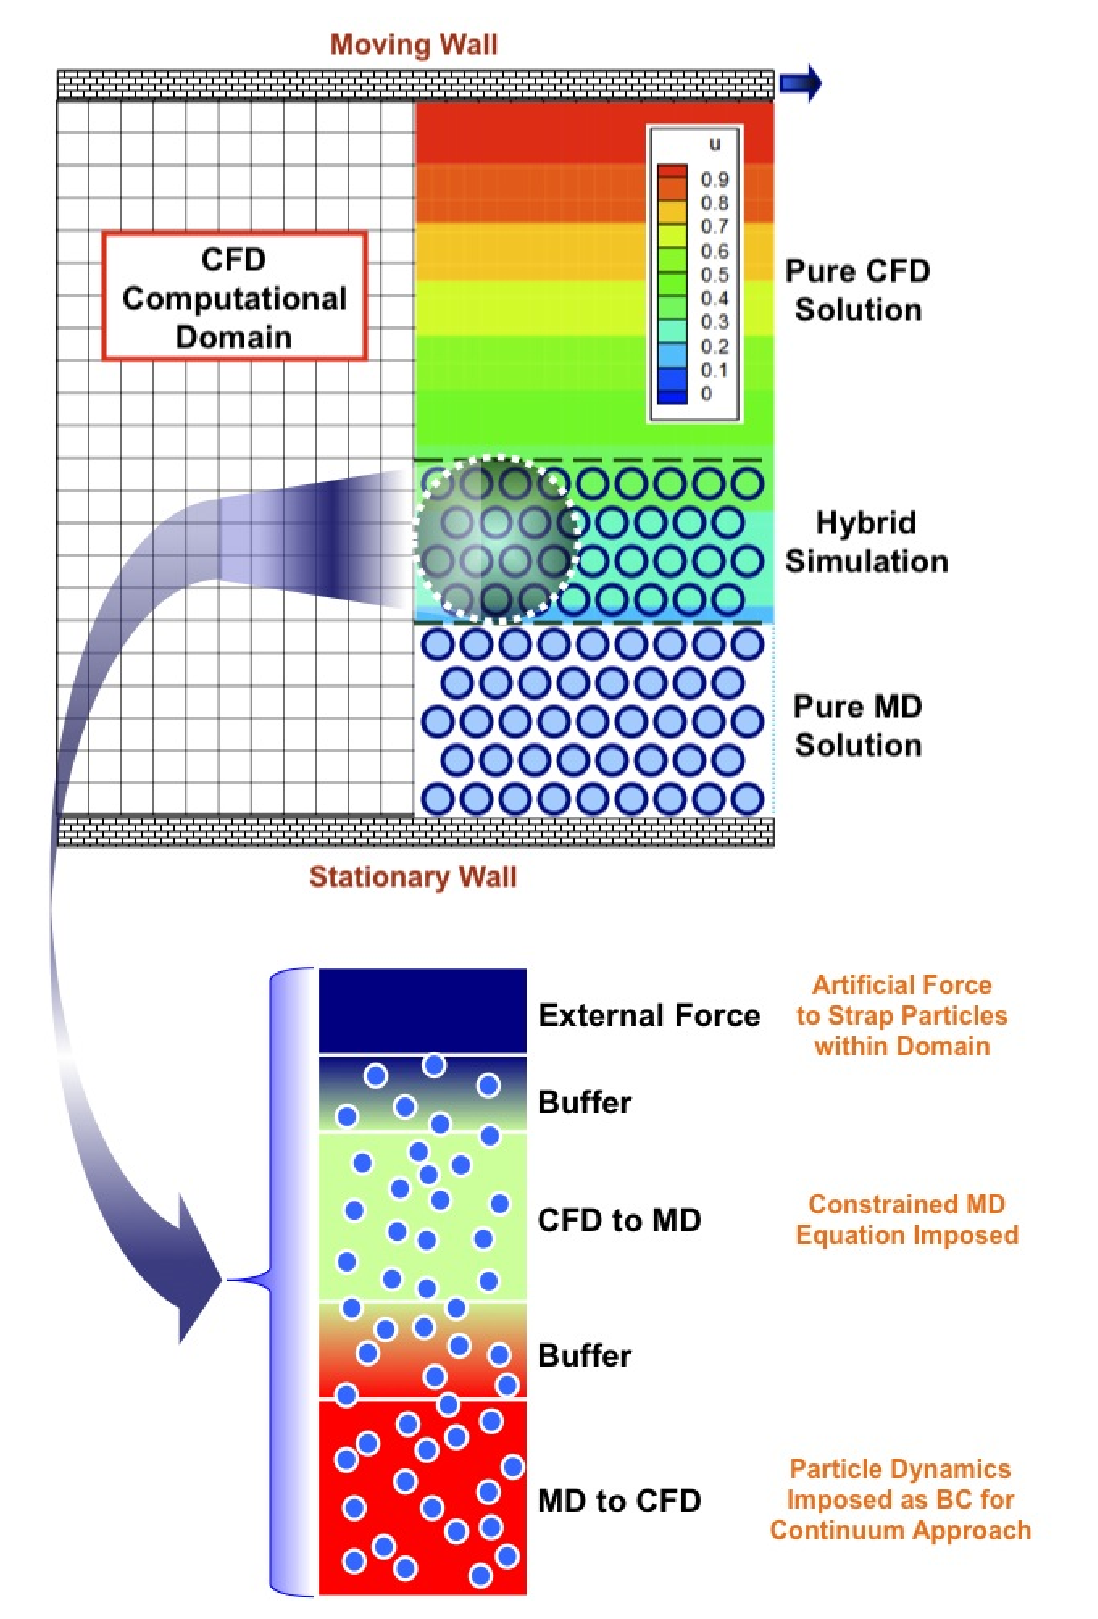
\includegraphics[scale=0.33]{fig1.eps}
%\linebreak
%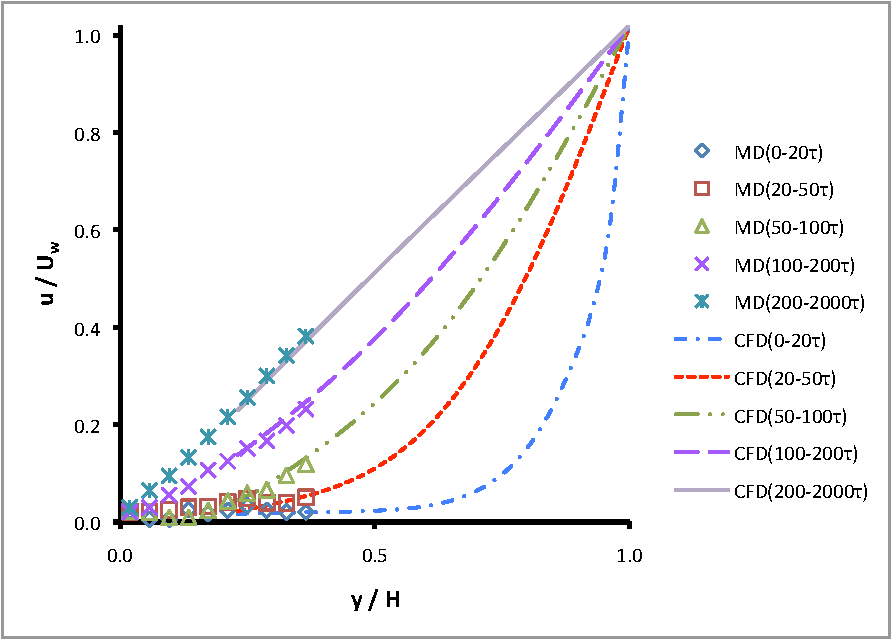
\includegraphics[scale=0.50]{Vel_Profile.PDF}
\caption{\small Schematic of CFD/MD Coupled Simulation of Channel Flow
  and the velocity profiles at different times \jhanote{should the
    graph be eliminated?}}
\label{Fig:Couette}
\end{figure}
%%%%% FIGURE %%%%%

In this study, we used the MPI version of the ``in-house''
incompressible CFD code~\cite{Lee} and the MPI version of the modified
version of LAMMPS~\cite{LAMMPS} for MD. We will present details of the
``in-house'' CFD code and the modifications that we made in LAMMPS
elsewhere~\cite{jocs_in_prep}. In brief, the hybrid region where the
coupling mechanism between MD region and CFD region is executed
comprises five sub-regions. In the CFD boundary grid region positioned
near the pure MD region, velocities of particles obtained with MD are
averaged and used for boundary condition for the corresponding CFD
computational cells. The MD boundary zone is placed above the CFD
boundary zone and here, information on velocities from the CFD grid
are imposed on particles in the zone through dynamically constrained
equation of motion for MD. As illustrated in Fig.~\ref{Fig:Couette},
the coupling mechanism is the key component for successful hybrid
CFD/MD simulations and our implementation follows the
literature~\cite{Nie},~\cite{Yen}.

% Between these zones, a buffer
% layer exists to avoid any harmful direct influences from one zone to
% another zone. The truncated and shifted Lennard-Jones potential is
% used for interactions of particles in MD simulation.

% To check the validity of the hybrid CFD/MD simulation, sudden-start
% Couette flow was employed that is similar to the test case used by
% O'Connell and Thompson~\cite{Thompson}.  The velocity profiles of
% hybrid approach are shown in the bottom of Fig.~\ref{Fig:Couette}. The
% line shows the velocity evolution which is solved by Navier-Stocks
% equations averaged over the given time intervals. MD results are shown
% as marks with same time intervals of CFD and overlap regions is
% indicated as both line and marks in the figure. These result is
% carried out for code validation of both CFD/MD and hybrid
% simulation. Good agreement between simulation results and analytical
% soluations.

As clearly indicated in Fig.~\ref{Fig:Couette}, the most prominent
computational challenge is how to run efficiently two separate stand
alone applications while efficiently conducting information exchange.
In other words, the time-to-solution is heavily dependent upon whether
a runtime environment can provide, (i) low collective-waiting times
(arising from batch queue wait times), and (ii) prevent an imbalances
in time to reach information exchange steps between the two codes. The
imbalance arises due to different performance between two distinctly
heterogeneous applications, CFD and MD, resulting in an unavoidable
time gap between arrival times of CFD and MD for the exchange step. We
propose to address this using dynamical resource allocation mechanism
with a load-balancing mechanism. In that sense, our SAGA-based
framework provides a single efficient runtime environment for the
coupled simulation.

%\Nkimnote{ }
%-------------------------------------------------------------------------
\section{SAGA and SAGA-based Frameworks for Large-Scale and Distributed Computation}

The Simple API for Grid Applications (SAGA) is an API standardization
effort within the Open Grid Forum (OGF)~\cite{ogf_web}, an
international standards development body concerned primarily with
standards for distributed computing. SAGA provides a simple,
POSIX-style API to the most common Grid functions at a sufficiently
high-level of abstraction so as to be %able to be
independent of the diverse and dynamic Grid environments. The SAGA
specification defines interfaces for the most common Grid-programming
functions grouped as a set of functional packages
(Fig.~\ref{Fig:SAGA1}). Some key packages are:

\begin{figure}[!ht]
 \begin{center}
     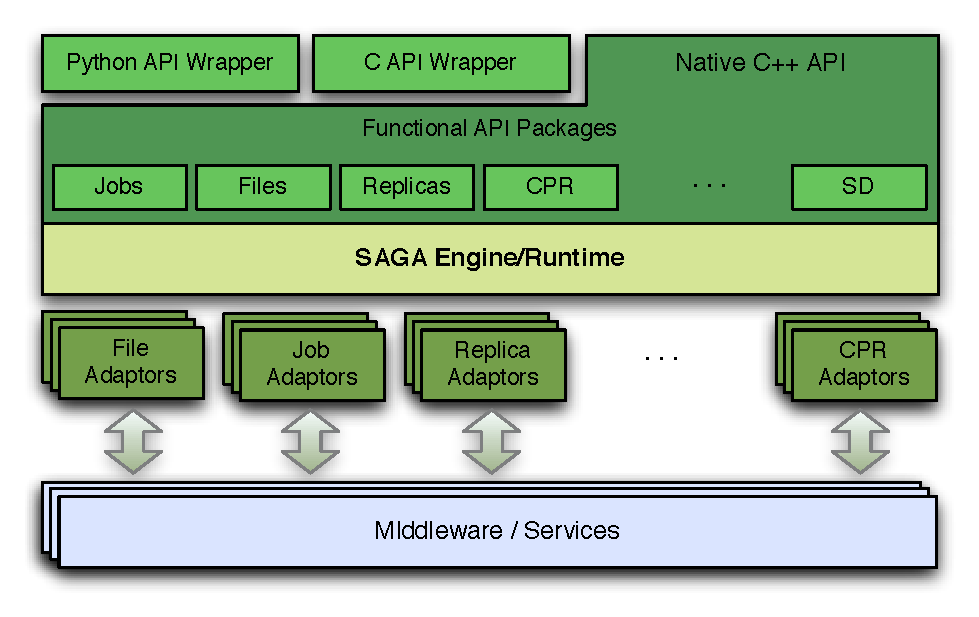
\includegraphics[width=0.40\textwidth]{stci_saga_figures-1.pdf}
 \end{center}
\caption{\small Layered schematic of the different components
  of the SAGA landscape. At the topmost level is the simple integrated API which provides the basic functionality for distributed computing. Our BigJob abstraction is built upon this SAGA layer using Python API wrapper} \label{Fig:SAGA1}
\end{figure}

%\begin{itemize}\addtolength{\itemsep}{-0.8\baselineskip}


\begin{itemize}
\item File package - provides methods for accessing local and remote
 filesystems, browsing directories, moving, copying, and deleting
 files, setting access permissions, as well as zero-copy reading and
 writing
\item Job package - provides methods for describing, submitting,
 monitoring, and controlling local and remote jobs. Many parts of
 this package were derived from the largely adopted
 DRMAA % ~\cite{drmaa_url}
 specification.
\item Stream package - provides methods for authenticated local and
 remote socket connections with hooks to support authorization and
 encryption schemes.
\item Other Packages, such as the RPC (remote procedure call) and Replica
 package
\end{itemize}


% \skonote{Introduction of PilotJob and BigJob (1 or 2 paragraphs) :
%   What is PilotJob, BigJob / what have been done so far and how
%   effective it was when using BigJob}

% \skonote{Joohyun, can you check this paragraph and improve it? In
%   this paragraph, I was going to talk about 'Structure and
%   Simulation Flow of BigJob Abstraction for Coupled Simulation'.}

Fig.~\ref{Fig:BigJob_Structure} shows the structure of BigJob and its
operation flow. When a BigJob is submitted to the remote resource, the
application manager monitors the status of this pilot-job through the
advert service. When resources are allocated to the BigJob, the
application manager divides obtained resources to its sub-jobs and a
coupled simulation starts under the control of a multi-physics agent
in the remote resource. Advert service keeps on getting the status of
a pilot-job from the queuing system and the status of sub-jobs from
multi-physics agent, also delivering these information to the
application manager by a push-pull mechanism. The application manager
watches the status of sub-jobs and decides the next event when the
coupled simulation is finished. When one default BigJob is launched,
subtasks keeps running until final solution is achieved and the
manager quits the pilot-job at that time. In cases multiple BigJobs
are submitted for the same simulation or a load balancing function is
included, sub-jobs experience several restarts from their
checkpointing data, reflecting changed processor allocation to each
application. In former case, resource allocation to each sub-job
follows a pre-defined map according to the number of BigJobs allotted
to this simulation: In latter case, resource allocation to each
sub-job becomes dynamic according to its performance, to be discussed
in the next section.

%%%%% FIGURE %%%%%
\begin{figure}
\centering
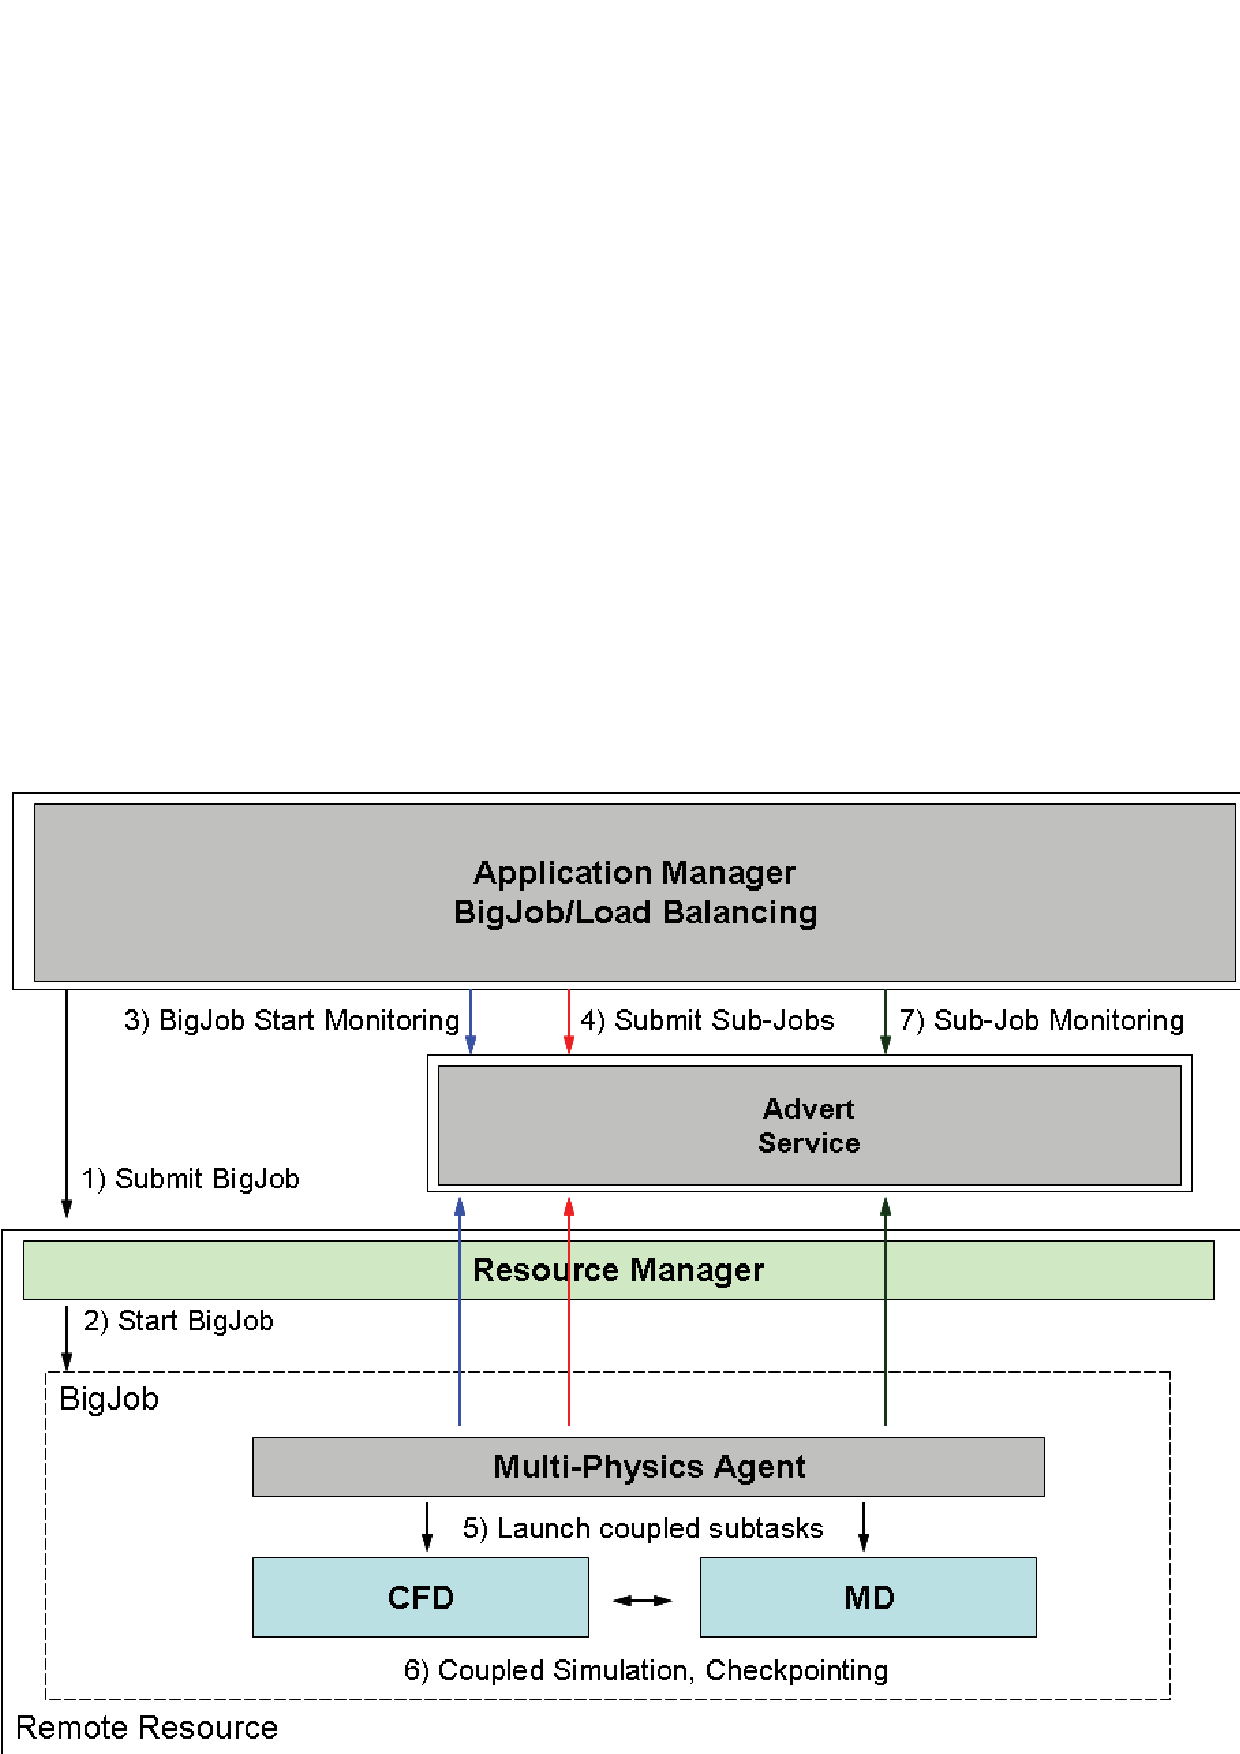
\includegraphics[scale=0.38]{Structure_of_BigJob}
\caption{\small Architecture of the Controller/Manager and Control
  Flow: Application manager is responsible for job management
  including BigJob and sub-job submission, their status monitoring
  functions. We implement a load balancing module, and migration
  service based on job information. Application agent system resides
  on each HPC resource and conducts job information gathering as well
  as communication with application manager via the advert service}
\label{Fig:BigJob_Structure}
\end{figure}
%%%%% FIGURE %%%%%



%-------------------------------------------------------------------------
\section{Load Balancing for Coupled Multi-Physics Simulation}

\jhanote{ALL: Please use code, simulations and applications
  consistently through the paper.}

% SAGA and its pilot-job framework (BigJob) enable coupled, yet distinct
% simulations to be submitted to queuing system. This is done by submitting one container
% job, and re-distributing its processors to each task. Also, total
% execution time can further be reduced by assigning more BigJobs and
% dynamically reallocating resources to each sub-task with increased
% number of processors. However, the

% As the current simulation requires frequent data exchange between
% CFD and MD during the simulation, it is likely to increase
% communication cost (strictly, waiting time for communication in one
% application) if their loads are not well balanced, which is quite
% different from former BigJob application~\cite{Jha:2009} where data
% exchange takes place when sub-tasks stopped temporarily.

% Meanwhile, checking sub-tasks' performances and controlling their
% operation for load balancing runs counter to SAGA's philosophy of
% "using services without changing the application source". Thus, help
% from application side is necessary to employ a load balancing
% function on a BigJob.

The flexibility to re-distribute resources (processors) to the
individual task, does not imply efficient utilization. This is the
responsibility of a load-balancer (LB) We will discuss the
implementation and algorithm of this LB; it is important to mention
that the LB functions in the context of the SAGA-BigJob framework.

Each application's load is determined by its elapsed time to run the
evolution loop. Here, time for initialization or inter-domain data
exchange are excluded from the counting, because they are one-time
event or irrelevant to application's performance.  The efficient
functioning of the LB is predicated on simulation codes being able to
restart from their checkpointing data effectively.  Also, simulations
should be equipped with generalized domain partitioning routine to run
simulation with any number of processors, without harming their
parallel efficiency a lot. If above conditions are satisfied, it makes
sense to load the LB within the pilot-job, to implement dynamic
resource allocation between tasks.  Conceptually, the load-balancing
algorithm assigns more processors to a sub-task with greater runtime,
until two codes take the same wall-clock time between points when they
communicate. Interestingly, our approach is very simple and the
algorithm is indepenendent of applications upon which it is predicated
are, (1) each application code follows the ideal parallel efficiency.
(2) all processors in one node are assigned to one single task.

Let the computation time (between exchanges) of the two simulations be
$t_{CFD}$ and $t_{MD}$, and the number of processors assigned to each
domain be $PE_{CFD}$ and $PE_{MD}$, respectively. Subscripts I and F
denotes initial and final states. Based on assumption (1), workload on
each application\jhanote{What does ``workload on each application
  mean''?} remains the same after the re-allocation of resources,
\begin{eqnarray}
W_{CFD} &=& PE_{CFD,I} \times t_{CFD,I} = PE_{CFD,F} \times t_{CFD,F} \nonumber \\
W_{MD} &=& PE_{MD,I} \times t_{MD,I} = PE_{MD,F} \times t_{MD,F}
\label{eq:SimTime_EachTask}
\end{eqnarray}
%\jhanote{Jeff: Please define what is $PE_{MD}'$, $t_{MD}'$} 
In spite
of re-allocation, the total number of processor utilized remains the
same:
\begin{equation}
%\begin{center}
PE_{TOT} = PE_{CFD,I} + PE_{MD,I} = PE_{CFD,F} + PE_{MD,F}
%\end{center}
\label{eq:PECondition}
\end{equation}
Our objective is to reduce the computation time of a subtask until the
two simulations show the same computation between the exchange points,
i.e., $t_{CFD,F} = t_{MD,F}$. From Equation~\ref{eq:SimTime_EachTask}
and Equation~\ref{eq:PECondition} an optimal processors distributed
for the CFD subtask would be:
%\jhanote{Jeff, please check this is correct} 
\begin{eqnarray}
PE_{CFD,F} & = & \frac {W_{CFD}} {(W_{CFD} + W_{MD})} \times PE_{TOT}
\end{eqnarray}

The MD simulation (sub-job) will follow a similar expression. 

The optimal processor distribution from above equation will return a
non-integer value. Also, under the second assumption (which is the
policy of many supercomputing centers), any load-balancing determined
as above, will proceed in discrete values determined by the number of
CPU cores in a node, which is denoted by $N_{UNIT}$.  \jhanote{the
  following is unecessarily complex. Simplify! Please remove
  everything and replace with one single sentence without any
  formulas. None of these terms are ever used again, so no point
  introducing terminology if never used again!!}

{\footnotesize{When upper and lower bound of $PE{CFD,F}$ is defined as
%\begin{boundval}
$ N_{UNIT} \times S \le PE{CFD,F} \le N_{UNIT} \times (S+1) $
%\end{boundval}
with $S = int(PE_{CFD,F} / N_{UNIT})$, either bound is going to
satisfy optimal processor distribution between CFD and MD tasks. CFD
computation time will determine coupled simulation time in the lower
bound ,whilst simulation time in the upper bound is dependent on MD
computation time, based on assumption (1). So, optimal processor
distribution is the one which satisfies smaller computation time
between $t_{CFD-in-Lower-Bound}$ and $t_{MD-in-Upper-Bound}$, who are
expressed by
\begin{eqnarray}
t_{CFD-in-Lower-Bound} & = & \frac {W_{CFD}} {N_{UNIT} \times S}
\nonumber \\
t_{MD-in-Upper-Bound} & = & \frac {W_{MD}} {PE_{TOT}-N_{UNIT} \times (S+1)}
\label{eq:Optimal_Time_Condition}
\end{eqnarray}
}}



%\hline
%\end{tabular}



%The control-flow within the BigJob Application-Manager when supporting a LB modules is shown in Fig.~\ref{Fig:BigJob_LB}. When one simulation loop is finished, the performance data of each subtask is sent to the load balancing module and it computes optimal resource distribution. Sub-job launcher restarts coupled application codes from their checkpointing data, according to the result of load balancing function. This process iterates until coupled simulation finalizes and processor allocation moves to the optimal condition during this process.

%%%%% FIGURE %%%%%
%\begin{figure}
%\centering
%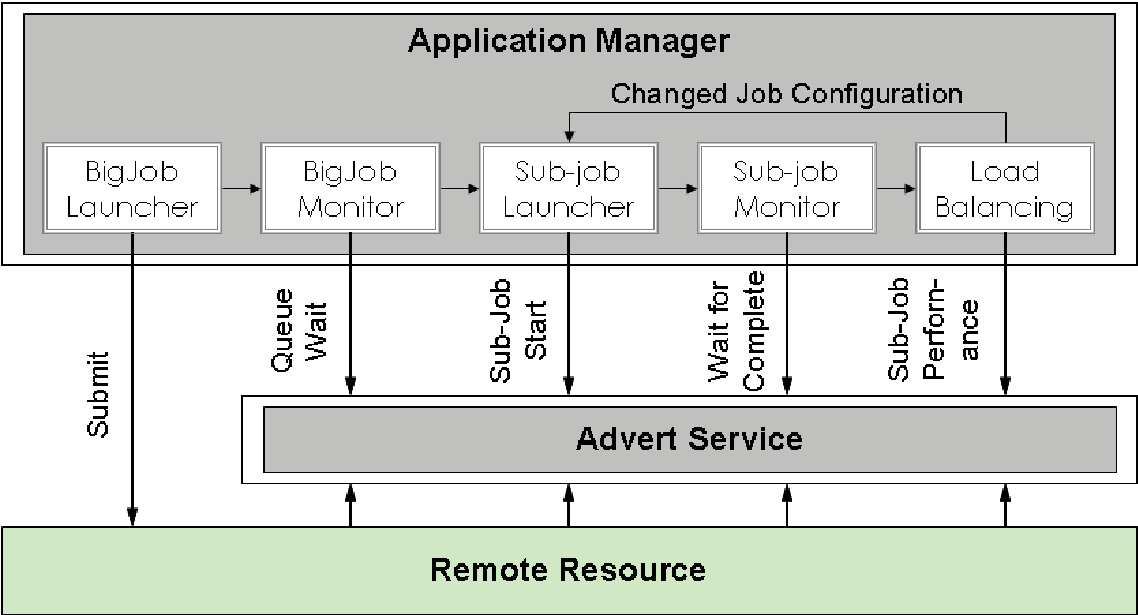
\includegraphics[scale=0.40]{BigJob_with_Load_Balance}
%\caption{\small Operation Flow of a BigJob with Load Balancing Function}
%\label{Fig:BigJob_LB}
%\end{figure}
%%%%% FIGURE %%%%%




%-------------------------------------------------------------------------
\section{Dynamic Resource Allocation for Coupled Simulations:
  Experiments and Analysis}

In Section 2, we outlined the challenges of running a coupled
multi-physics simulation using conventional queuing system as, (i)
Difficulty of starting multiple applications concurrently; (ii)
Inability to balance the load among domains, and (iii) Fixed number of
allocated resources throughout the simulation. To address these
challenges we use the BigJob abstraction with a load balancing module
for dynamic resource allocation.

% \skonote{Need to check section 2, whether we have mentioned the
%   necessity of BigJob. This includes why we need BigJob, rather than
%   unifying application codes. Here, we should mention that 'minimizing
%   the application code change is the SAGA's great benefit'.}

% With the ultimate aim of reducing the total simulation time, we
% investigate acquiring idle resources during the simulation, by
% launching multiple BigJobs for one coupled simulation.

We outline three different scenarios that arise. In the first
scenario, a single BigJob is utilized to run the coupled-simulations,
with (S1-LB) and without (S1) LB redistributing resources based upon
their individual performance.  In the second scenario (S2) there are
two BigJobs, and although they are started together, most often one
BigJob starts before the other; to increase efficiency, both coupled
simulations start with whatever resources are available as part of the
first (to run) BigJob. When the second BigJob becomes active, there is
a dynamic redistribution of tasks, such that the larger of the two
simulations is assigned the bigger BigJob. Variant of the above, when
the two BigJobs are on different machines forms the third scenario
(S3). In the remainder of this section we discuss the details of these
three different Use Cases.

% We compare the performance as measured by TTS using the benchmark
% case to be the situation when we do not have the ability to utilize
% the BigJob concept and thus each simulation interacts with the
% queueing system differently, and thereby each must be in an Active
% state before both can start running.

% \jhanote{please be sure to use co-scheduling where appropriate and
%   not concurrency}

\skonote{Included a new subsection, to describe how the experiments are performed.}
% \subsection{Description of Experiments}
% A simple couette flow, which is depicted on Figure 1 in Section 2,
% is simulated to validate the runtime reduction by applying BigJob
% abstraction on CFD-MD coupled simulation. The current flow system is
% composed of 62,400 mesh points in CFD side and 23,188 particles in
% MD side, both of which are such a small system in each scientific
% domain. This coupled simulation runs for 2500 $$\tau$$ physical time
% to get a converged solution, which is equivalent to 25,000
% iterations on CFD code and 500,000 iterations on MD code. During the
% simulation, both codes update their boundary values by exchanging
% their simulation data through file-based approach, once in every 10
% $\tau$. This leads to 250 times synchronization between two
% application domains throughout the simulation.  A coupled simulation
% by the default one BigJob does not require any change of application
% codes. On the other hand, it is inevitable to have application codes
% changed to use advanced functions such as the load balancing between
% coupled codes or to get assigned with more resources during
% simulation, because SAGA does not have any control over application
% sides. First, in both cases, application codes need to have an
% application-level checkpointing and generalized domain partitioning
% method with any number of processor allocation. As the new resource
% assignment between two domains by a load balancing function or a new
% BigJob allocation can be applied when the simulation is temporarily
% stopped, application codes need to stop several times and restart
% from its checkpointing data with changed number of processors
% assignment. In the current test, application codes stop and restart
% from checkpointing data on every 500 $\tau$, which is the same as
% 1/5 of total iterations. Second, to use a load balancing function,
% application codes need to return their actual computation time data
% to the BigJob. This is far different from each application's
% simulation time, which can be monitored by the BigJob: One-time
% event such as domain partitioning or checkpointing, and waiting time
% between application domains which is going to be minimized as they
% are well-balanced, should be excluded from the consideration of
% application's performance. In the current test, CFD and MD codes
% have several time checking functions inside to capture total
% iteration time without inter-domain information exchange.  All these
% tests were conducted on supercomputing resources on LONI (Louisiana
% Optical Network Initiative)~\cite{LONI_web} resources and their
% specifications are listed on table~\ref{table:LONI_resource}. As
% given on the table, QueenBee system is far larger than other
% resources in total number of processors, while all the others are
% identical. Based on our monitoring over these systems, QueenBee has
% been very crowded while all others have been less occupied. Thus,
% tests on small systems are focused on quantifying runtime reduction
% by using the BigJob abstraction, while tests on QueenBee is rather
% involved in arguing the benefit of co-scheduling on crowded
% systems. wall-time limit is set to be 6 hours in all tests, which
% seems enough for the active simulation and inactive idling, i.e.,
% the time between the first job and second job allocations in
% conventional job submission.

\subsection{Description of Experiments}

Fig.~\ref{Fig:OneBJ_Flow} shows two different scenarios: the first
(leftmost) shows the time evolution of a coupled simulation with the
conventional job submission and through one BigJob. In a conventional
way, individual tasks with resource requirements of $PE_{CFD}$ and
$PE_{MD}$, respectively, are independently submitted to the
conventional queuing system and job scheduler recognizes these coupled
tasks as two distinct jobs. Thus, they are going to start at a
different time, except when enough resources are available. In this
case, both tasks wait on the queue when no job is allocated, the first
allocated job idles to do data exchange with its counterpart, and run
actual simulation after both jobs are allocated. On the other hand, in
S1, a pilot job \jhanote{change to BigJob!} of size $PE_{CFD}+PE_{MD}$
is submitted to the queue, and coupled simulation directly starts when
the resource is assigned on this BigJob.  ... inactive mode in
conventional job submission, while total runtime is the same if the
resource distribution to sub-jobs is identical. However, eliminating
inactive mode does not guarantee total simulation time is reduced,
because waiting to get one bigger allocation may happen to take more
than getting two allocations with smaller chunks. The same situation
can happen to the load-balanced case with one BigJob, which satisfies
the reduction of total runtime compared to other examples.
Figure~\ref{Fig:TwoBigJobs} illustrates scenarios S2 and S3 -- whereby
2 BigJobs are submitted as opposed to 1 BigJob. In S2 both BigJobs are
on the same machine, whilst in S3 they are on different machines.  As
we will show later, under certain load and queue conditions, it is
possible that two smaller BigJobs -- either S2 or S3, begin sooner
than a larger subtask (S1).

%%%%% FIGURE %%%%%
\begin{figure}
\centering
\includegraphics[scale=0.40]{Simulation_Time_of_One_BigJob.eps}
\caption{\small Comparison of dependencies encountered for
  coupled-simulations submitted as conventional Jobs, to the scenario
  when using Pilot-Jobs (BigJob). Here we use only 1 BigJob. The
  conventional mode of submission experiences three phases of queue
  waiting (all jobs are waiting: $t_1-t_0$), inactive mode (one job is
  waiting for another: $t_2-t_1$), and active running (running a
  coupled simulation: $t_f-t_2$). On the other hand, inactive mode
  disappears when coupled simulation runs within one BigJob, as an
  allocated BigJob distributes its resource to sub-jobs.}
\label{Fig:OneBJ_Flow}
\end{figure}
%%%%% FIGURE %%%%%


% While we investigate the benefit of co-scheduling and load balancing
% on coupled distinct tasks in a single BigJob scenario, which is
% rather inclined to efficiently utilizing the computing environment
% within system's default configuration, we rather focus on physically
% increasing system's usage in next scenarios.  \skonote{Prof.Jha, can
%   you correct the above sentence? Intention was, 'while one BJ uses
%   computers efficiently within default system setup like queueing,
%   using two or more BJs will increase real usage of CPUs, thus
%   maximizing the use of idling resources.'}



% runtime environment for coupled multi-physics simulations would
% benefit from dynamic resource availability exploited by BigJob
% implementation. It is possible to assign more CPUs for a slowing
% application when another BigJob becomes available.  Compared to S1
% for a coupled simulation in Figure~\ref{Fig:OneBJ_Flow}, faster
% start of coupled subtasks. Also, when next BigJob is also allocated
% to this coupled simulation, total job size will be the same as one
% BigJob submission. Resource allocation and simulation flow is
% identical to the conventional job submission, but inactive idling in
% a conventional case disappears as a BigJob framework starts coupled
% subtasks with smaller number of processors when first job is
% allocated. So, submitting two BigJobs guarantees the reduction of
% total simulation time compared to conventional job submission, if
% all conditions are identical. If this two BigJob submission is
% applied on multiple sites, it is more likely to get two allocations
% faster than requesting two jobs in the same site. However, faster
% launch of two BigJobs does not guaranteed save of total simulation
% time, because time for data exchange between applications will also
% increase if distributed resources cooperate.


%%%%% FIGURE %%%%%
\begin{figure}
  \centering \includegraphics[scale=0.40]{Simulation_Time_of_Two_BigJobs.eps} \caption{\small
    Schematic comparing the distribution of simulations when 2 BigJobs
    are used, first on the same physical machine, then on different
    (distributed) machines. In both cases, coupled sub-jobs start
    running when the first BigJob is allocated at $t=t_1$ and
    experience resource reallocation with increased amount when the
    next BigJob becomes available. When two BigJobs are allocated,
    each sub-job occupies one BigJob and data exchange between jobs
    takes place across BigJobs.}  \label{Fig:TwoBigJobs} \end{figure}
%%%%% FIGURE %%%%%

We investigate a simple couette flow (Fig.~\ref{Fig:Couette}) as the
representative physical problem, to validate the performance gains and
resource flexibility of above scenarios.
%arising from the Pilot-Job based approach.
%by applying BigJob abstraction on CFD-MD coupled simulation.
The current flow system is
composed of 62,400 mesh points (CFD) and 23,188 particles (MD).
% both of which are such a small system in each scientific
% domain. 
In order to reach convergence, the coupled simulation runs for a
physical time of 2500$\tau$, which is the time unit related to the
characteristics of molecules. This is equivalent to 25,000 CFD
iterations and 500,000 MD integration steps. During the simulation,
both codes components update their boundary values by exchanging their
simulation data via files, once every 10 $\tau$. This leads to 250
synchronization steps between two simulation components over the
course of a single simulation run. For a rigorous test of a load
balancer, larger coupled simulation task (which has 150 times more
workload on CFD domain and 50 times on MD) also has been
experimented. The wall-time limit of all simulations are set to 6
hours, which is large enough to encounter both the active and inactive
phase experienced in conventional job submission. In the larger
simulation, wall-limt time is increased to 24 hours, consdiering its
runtime which is around 11 hours.

No changes in the simulation codes were required in order to utilize
the BigJob capabilty; however, in order to utilize load-balancing
features or dynamic-resource assignement the simulation codes need to
be equipped with the ability to carry out application-level
checkpointing.  The application codes in addition to having
application-level checkpointing need generalized domain partitioning
method to work with a range of processor counts. In the current work,
the application codes experience five launch/re-launches (25 times in
larger simulation) to get assigned with changed number of processors,
either by the result of load balancing or more resource allocations.

% A coupled simulation by the default one BigJob does not require any
% change of application codes. On the other hand, it is inevitable to
% have application codes changed to use advanced functions such as the
% load balancing between coupled codes or to get assigned with more
% resources during simulation, because SAGA does not have any control
% over application sides. 

% For example, with a new resource assignment, 
% a load balancing function or a new BigJob allocation can be
% applied when the simulation is temporarily stopped, application codes
% need to stop several times and restart from its checkpointing data
% with changed number of processors assignment. 

The use of a load balancing function requires one more change on
application codes. As load balancer refers to the performance data
from application codes, application codes need to return their actual
computation time, which excludes idle waiting on inter-domain
information exchange. This can be implemented by checking elapsed time
on inter-domain data exchange and subtracting it from total iteration
time.
%\jhanote{I'm not  sure I understand the following}
One-time event such as domain partitioning or checkpointing, and
waiting time between application domains which is going to be
minimized as they are well-balanced, should be excluded from the
consideration of application's performance.
%e architected the CFD and MD codes to have several
time checking functions inside to capture total iteration time without
inter-domain information exchange.


Simulations used to validate and determine performance values were
conducted on supercomputing resources on TeraGrid machines (62,976
cores Ranger), shared TeraGrid-LONI (Louisiana Optical Network
Initiative)~\cite{LONI_web} resources including Queenbee(5,440 cores)
and some smaller LONI clusters such as Eric, Oliver, Louie and
Poseidon(512 cores).  We monitored the load on these systems over a
long period of time (several weeks) and found Queenbee to be
significantly more loaded than other resources.

% \jhanote{Do we still want the following sentence?} Thus, tests on
% small systems focus on quantifying runtime reduction by using the
% BigJob abstraction, while tests on QueenBee is rather involved in
% arguing the benefit of co-scheduling on crowded systems.

\jhanote{I don't understand the next sentence:} The status of the
systems are predicted using load factor through the ratio of the
number of nodes in active jobs over the total number of nodes when the
job had been submitted. \jhanote{The following is out of place:} The
load factor was recorded on every job submission by changing of the
requesting number of processor from 8 to 64 and the requesting
wall-time limit from 1 hr to 12 hr. Order of job execution depends on
a variety of parameters such as submission time, backfill
opportunities, number of actively scheduled jobs and queue priority
including credential, fairshare, resource and service priority. The
result of simulation actual waiting time via queuing system shows very
diversity and variance as a matter of course.

% monitoring over these systems, QueenBee has been very crowded while
% all others have been less occupied.

\subsection{Using Pilot-Jobs to submit Coupled Simulations:
  Performance Analysis}

We wanted to see if we could come up with an analysis that would tell
us how running larger and/or longer simulations effects the actual
waiting time on the queue.

\Nkimnote{Will be added some two small job Vs. BigJob table here}

\begin{table}[t]
  \caption{\small  Effect of various configurations on waiting
time. The tables show the actual waiting time on the queue with
respect to the changing number of processors and different wall-time
limits when jobs were submitted on Ranger and Queenbee.  Comparing the
actual waiting time with the number of processors on each wall-time
limit, quantitative tendency of waiting times is to somewhat decrease
when requested number of processors increases. But the relationship
between the waiting time and wall-time limit was hardly observed.
However, these works constitute a good case study for showing variance
of actual waiting time on the queueing system.}
\label{table:waitingtime}
\centering
\begin{tabular}
{p{0.4in} || p{0.4in} p{0.4in} p{0.4in} p{0.4in} p{0.4in}}
\multicolumn{6}{c}{\phantom{\tiny 100}}\\
\hline
%\midrule
 \multirow{3}{0.4in}{number of processors}&
 \multicolumn{5}{c}{wall-time limit with 92$\pm$6\% workload (Ranger)}
\\
\cline{2-6}
%\cmidrule{2-6}
 & \nyc 2hr
 & \nyc 3hr
 & \nyc 4hr
 & \nyc 6hr
% & \nyc 6hr
& \multicolumn{1}{c}{12hr}
%  &1hr &2hr &4hr &6hr &12hr
\\
\cline{2-6}
%\cmidrule{2-6}
 &\multicolumn{5}{c}{Waiting time on the queue [sec]}
\\
\cline{1-1}
%\cmidrule{1-1}
\nyc 16
 & \nyc 9989 & \nyc 15984 & \nyc 39151 & \nyc 65 & \multicolumn{1}{c}{66}
\\
\nyc 32
 & \nyc 15371 & \nyc	4106 & \nyc 11376 & \nyc 54 & \multicolumn{1}{c}{55}
 \\
\nyc 48
  & \nyc 13264 & 4392 \nyc  & \nyc 37780 &\nyc 43 & \multicolumn{1}{c}{44}
\\
\nyc 64
 & \nyc 9944 &	\nyc 1975	 & \nyc 39855 & \nyc 31 & \multicolumn{1}{c}{32}
\\
\hline
%\midrule


\multicolumn{6}{c}{\phantom{100}}\\
\hline
%\midrule
 \multirow{3}{0.4in}{number of processors}&
 \multicolumn{5}{c}{wall-time limit with 95$\pm$4\% workload (Queenbee)}
\\
\cline{2-6}
%\cmidrule{2-6}
 &\nyc 2hr
 &\nyc 3hr
 &\nyc 4hr
 &\nyc 6hr
 &\multicolumn{1}{c}{12hr}
\\
\cline{2-6}
%\cmidrule{2-6}
 &\multicolumn{5}{c}{Waiting time on the queue [sec]}
\\
\cline{1-1}
%\cmidrule{1-1}
\nyc 16
 & \nyc 14339 & \nyc 3578  & \nyc 39113 & \nyc 6 & \multicolumn{1}{c}{940}
\\
\nyc 32
 & \nyc 14312 & \nyc 3550 & \nyc 39238 & \nyc 5 &\multicolumn{1}{c}{6344}
 \\
\nyc 48
 & \nyc 21555 & \nyc 3517 & \nyc 39207 & \nyc 4 & \multicolumn{1}{c}{6353}
\\
\nyc 64
 & \nyc 21541 & \nyc 3489 & \nyc 39179 & \nyc 3 & \multicolumn{1}{c}{6329}
\\
\hline
%\midrule
\end{tabular}
\end{table}

What we did was the following. We chose two machines with more than
5000 processors, Ranger and Queenbee. We submitted jobs of different
sizes, requiring different wall-time limits. Each time we submitted a
job, we gathered the load factor and the actual waiting time on the
queue. Lots of factors effect the waiting times. Most important of
them is the load at the moment on the machine, requested wall-time
limit and also the number of processors requested. Two more factors
that effect this are the backfilling that occurs when some other
irrelevant job ends and the changes in the priority of our own job
when a particular higher priority job joins the queue.  The waiting
time has a tendency to decrease as the number of processors of a job
increase, as can be seen from Table~\ref{table:waitingtime}.
Considering only the data from the jobs which did not go through
backfilling, it can be seen that larger processor jobs start earlier
based on the priority of jobs.

We cannot claim this just by running some tests on a couple of
machines. It may be, in part, due to the policies and loads under
which a particular machine is run. The waiting time has a little
relationship with wall-time limit of jobs. But from experience, we
feel that running a large job is better than running two smaller
jobs. We say that the sum total of the waiting times of two smaller
jobs is going to be larger than the waiting time of a single large
processor job. This is especially true in cases where the jobs need to
interact.

\jhanote{This section needs to establish the basic feature that on
  average, over different loads and on different machines that
  submitting larger simulations is beneficial, i.e., lowers the \ts.}

\skonote{Jeff's edit from here}

% \begin{table}[t]
% \caption{\small  Effect of various configurations on waiting time. The tables show the actual waiting time on the queue with respect to the changing number of processors and different wall-time limits when jobs were submitted on Ranger and Queenbee. 
% Comparing the actual waiting time with the number of processors on each wall-time limit, quantitative tendency of waiting times is to somewhat decrease when requested number of processors increases. But the relationship between the waiting time and wall-time limit was hardly observed.
% However, these works constitute a good case study for showing variance of actual waiting time on the queueing system.
% }
% \label{table:waitingtime}
% \centering
% \begin{tabular}
% {p{0.4in} || p{0.4in} p{0.4in} p{0.4in} p{0.4in} p{0.4in}}
% \multicolumn{6}{c}{\phantom{\tiny 100}}\\
% \hline
% %\midrule
%  \multirow{3}{0.4in}{number of processors}&
%  \multicolumn{5}{c}{wall-time limit with 92$\pm$6\% workload (Ranger)}
% \\
% \cline{2-6}
% %\cmidrule{2-6}
%  & \nyc 2hr
%  & \nyc 3hr
%  & \nyc 4hr
%  & \nyc 6hr
% % & \nyc 6hr
% & \multicolumn{1}{c}{12hr}
% %  &1hr &2hr &4hr &6hr &12hr
% \\
% \cline{2-6}
% %\cmidrule{2-6}
%  &\multicolumn{5}{c}{Waiting time on the queue [sec]}
% \\
% \cline{1-1}
% %\cmidrule{1-1}
% \nyc 16
%  & \nyc 9989 & \nyc 15984 & \nyc 39151 & \nyc 65 & \multicolumn{1}{c}{66}
% \\
% \nyc 32
%  & \nyc 15371 & \nyc	4106 & \nyc 11376 & \nyc 54 & \multicolumn{1}{c}{55}
%  \\
% \nyc 48
%   & \nyc 13264 & 4392 \nyc  & \nyc 37780 &\nyc 43 & \multicolumn{1}{c}{44}
% \\
% \nyc 64
%  & \nyc 9944 &	\nyc 1975	 & \nyc 39855 & \nyc 31 & \multicolumn{1}{c}{32}
% \\
% \hline
% %\midrule


% \multicolumn{6}{c}{\phantom{100}}\\
% \hline
% %\midrule
%  \multirow{3}{0.4in}{number of processors}&
%  \multicolumn{5}{c}{wall-time limit with 95$\pm$4\% workload (Queenbee)}
% \\
% \cline{2-6}
% %\cmidrule{2-6}
%  &\nyc 2hr
%  &\nyc 3hr
%  &\nyc 4hr
%  &\nyc 6hr
%  &\multicolumn{1}{c}{12hr}
% \\
% \cline{2-6}
% %\cmidrule{2-6}
%  &\multicolumn{5}{c}{Waiting time on the queue [sec]}
% \\
% \cline{1-1}
% %\cmidrule{1-1}
% \nyc 16
%  & \nyc 14339 & \nyc 3578  & \nyc 39113 & \nyc 6 & \multicolumn{1}{c}{940}
% \\
% \nyc 32
%  & \nyc 14312 & \nyc 3550 & \nyc 39238 & \nyc 5 &\multicolumn{1}{c}{6344}
%  \\
% \nyc 48
%  & \nyc 21555 & \nyc 3517 & \nyc 39207 & \nyc 4 & \multicolumn{1}{c}{6353}
% \\
% \nyc 64
%  & \nyc 21541 & \nyc 3489 & \nyc 39179 & \nyc 3 & \multicolumn{1}{c}{6329}
% \\
% \hline
% %\midrule
% \end{tabular}
% \end{table}

% \skonote{Jeff's edit till here}



\subsection{Scenario S1: Pilot-Job with Load Balancing}

\jhanote{Do not have such long paragraphs. One paragraph should
  represent one simple compact idea. Maxm of 4-5 sentences!!}

Figure~\ref{Fig:Queuewait_LONI} and table~\ref{table:oneBJ_Test} show
queue waiting and job simulation time performed on small LONI
resources, running above test cases: conventional job submission, one
default BigJob launch and one BigJob with load balancing. A coupled
simulation has been conducted by using 32 and 64 processors, with the
same number of processors allocated to CFD and MD
subtasks. Simulations are restarted after load-balancing four times
using checkpointing data. The waiting time until the launch of a
coupled simulation is shown in figure~\ref{Fig:Queuewait_LONI}. From
the graph \jhanote{Figure 6 is not a graph} the waiting time (or
waiting time and inactive mode in conventional testsuites) did not
show a close relationship with the workload of the system \jhanote{has
  workload been defined? If not, define before this. If yes, remove!!}
(which is defined as the sum of number of processors either running or
waiting on the queue before the current job submission, divided by
total number of processors in the system). Even some cases when
workload is bigger than 1, all simulations experienced the direct
start of a simulation by the help of a backfill capacity. Though a
BigJob simulation had more possibility to start faster than either of
submitted tasks through the conventional way, some test cases also
showed that the conventional coupled simulation was starting ahead of
a BigJob simulation.  Meanwhile, the detailed analysis over the above
data shows that the use of a BigJob gives a great benefit on coupled
simulation, both in terms of faster start and job stability. Regarding
the faster start, the job queueing priority on many supercomputer
systems usually allow a bigger job to get higher priority, letting one
BigJob start faster than any of independently submitted tasks in
normal condition. Even in cases conventional job started coupled
simulation faster than a BigJob launch, most events happened not
because these smaller jobs get the benefit of a backfill capability
twice before the start of a BigJob, but because direct job submission
on the system filled available resources before a BigJob submission
passing through the advert server arrives in the system. Especially,
even with the sufficient wall-time limit on job submission, a
conventional job submission showed an event of job failure due to the
time over of first allocated task. As the BigJob submission is free
from this inactive waiting, wall-time limit can be far reduced than
conventional job submission and this would increase BigJob's
possibility to be allocated by a backfill capability.

%%%%% FIGURE %%%%%
\begin{figure}
\centering
\includegraphics[scale=0.40]{Simulation_Time_of_One_BigJob.eps}
\caption{\small Waiting time of a conventional job submission and a
  BigJob submission, with 32 and 64 processors on LONI's local
  resources: Eric, Oliver, Louie and Poseidon. Job start time in
  conventional job submission is denoted by X: the line between two
  symbols represent the inactive waiting of a first launched job. O
  symbol represents the start time of a BigJob submission. X axis
  means the workload and Y axis is waiting time, presented by a log
  scale. Conventional job submission and one BigJob tests were
  conducted by 12 times.}
\label{Fig:Queuewait_LONI}
\end{figure}
%%%%% FIGURE %%%%%

\setlength{\tabcolsep}{1pt}
\begin{table}[!ht]
\begin{center}
 \caption{\small Results for performance data using BigJob with and
    without LB. The baseline simulation represents the case when
    BigJob is not used; in this case, the time to start is dominated
    by the Inactive Mode of the longer waiting task. The use of BigJob
    resolves, this as can be seen by the reduced inactive mode time in
    columns 3 and 4. The starting configuration assigns resources
    equally between CFD-MD -- 16px each. However, after a few
    iterations of the LB the configuration is 8-24. With this
    configuration the performance is better with LB, than without
    LB 1370 $\pm 98$ vs 1641 $\pm$ 162. The starting configuration
    of the second set (8-24) is a ``balanced configuration'' which is
    why there is no performance gains on using the LB. Values in table
    shows averaged time in seconds, values within a parenthesis are
    standard deviation of time elapsed; the average is taken over 5
    distinct experiments. \jhanote{use S1 and S1-LB}}
% experiments. }
%\label{table:systems}
\label{table:oneBJ_Test}

\begin{tabular}{ c|| c | c }

\hline
16-16 & Active Runtime & Time for Iterative Loop \\
\hline
\hline
Conventional & 1448    & 1349 \\
Submission   & (13)    & (41) \\
\hline
BigJob     & 1458    & 1365 \\
(no LB)    & (59)  & (15)\\
\hline
BigJob     & 1294    & 967 \\
(LB)    & (54)  & (21) \\
\hline
\hline
\end{tabular}


\begin{tabular}{ c|| c | c }
\hline
\hline
32-32 & Active Runtime & Time for Iterative Loop \\
\hline
\hline
Conventional & 861    & 741 \\
Submission   & (65)    & (47) \\
\hline
BigJob     & 892    & 759 \\
(no LB)    & (89)  & (26)\\
\hline
BigJob     & 969    & 617 \\
(LB)    & (111)  & (47) \\
\hline

\end{tabular}
\end{center}
\end{table}


The result of simulation runtime is shown in the
table~\ref{table:oneBJ_Test}. From the result in tests with 32
processors, a conventional job submission and one default BigJob
running show nearly the same computational cost, while one BigJob
simulation with LB shows better performance on runtime. Load balancing
function changes the resource distribution to the best condition after
the first simulation loop and 8 processors from CFD task are moved to
MD simulation from the next start. From the next start, the processor
distribution between subtasks remains the same. As a result, total
runtime is saved by about 10 percent compared to other test cases. On
the other hand, a load balanced BigJob shows worse performance when 64
processors are used on simulation, by around 10 percent compared to a
conventional job submission. In this case, a load-balanced BigJob
initially starts with same number of processors to each subtask,
slowly moving to assign more resources on the MD side, until finally
12 processors are allotted to CFD simulation. In both tests, a default
one BigJob experiences slightly worse performance compared to the
computation time on a conventional case.  Above result of simulation
performance can be discussed as follows. At first, worse performance
of a default BigJob is caused by the additional cost on running a job
through advert server and monitoring the status of a BigJob. Because
of the frequent monitoring, a coupled task even experiences the
increase of a simulation time on solving the iterative
loop. Meanwhile, the bad performance on a load-balanced BigJob is
because of multiple reasons. Aside from above issues, the
load-balanced BigJob experiences the redundant cost on restarting
application codes, when they have to reinitialize and load the
checkpointing data. In both test cases, a load-balanced BigJob has
spent about three times more cost on one-time event during the
simulation (which can be gained by the subtraction between total
computation time and iteration time). This is closely related to the
checkpointing and restarting interval. Also, the algorithm itself
needs to be refined to predict the performance of each code more
precisely. In the simulation with 32 processors, a load balancer
computed the optimal ratio of processor distribution to be 8 to 24
between CFD and MD tasks, based on the computation time in this
assignment, which takes 108 seconds on CFD and 194 seconds on MD
simulation. Because of the assumption that all applicatio ncodes will
experience the ideal parallel efficiency, a load balancer determines
that the current resource distribution is better than the other

\skonote{Will correct the caption in the below table.}



\subsection{Scenario S2 and S3: Logically and Physically Distributed
  Pilot-Jobs}


In Table~\ref{table:TwoBigJobs}, test measurements for performance
gains are summarized. The scenario for this testing is simple for
clarifying benefits. Initially, two BigJobs are submitted to one HPC
resource or two HPC resources. Once the first bigjob becomes
available, two applications are submitted as two subtasks with
pre-defined cpus to the bigjob, and then when another bigjob becomes
available later, two subtasks for each application is reconfigured by
assigning the entire cpus of a bigjob to one application. Table
~\ref{table:TwoBigJobs} shows performance gains with such a scenario
in terms of MD run time since CFD run time is always smaller under
this setting. In this simple scenario, other complicated aspects such
as file transfer, in particular between two distributed resources are
not considered but in the future study, the overall performance will
be optimized by considering them.

% Performance gains with two bigjobs. Performance is measured with CPU
% times consumed by MD, since test cases we used always require longer
% cpu times for MD than those of CFD.  Performance gains with
% additionally available bigjob can be seen by comparing MD CPU times
% with those obtained with the initial bigjob.  Measurements were
% carried out with LONI cluster systems.  louie and poseidon are dell
% cluster systems having 128 nodes with 4 cores in a
% node. \jhanote{add bigjob size --- which 8 and 16} Test 1 and 2
% correspond to Use Case 2; Test 3 and 4 correspond to Use Case 3
% \newline }

\begin{table}[!h]
\begin{center}
\caption{\small Performance measures for Use Case 2 and 3.  The general scenario for these cases is that one bigjob is launched first and the other bigjob becomes available later in the same system (Use Case 2) or the remote system (Use Case 3).  Results are presented with four test cases (two cases for each Use Case 2 and 3, respectively) and demonstrate a performance gain with the additionally available bigjob. Here, we present the time to solution in terms of two components, ${T_{comm}}$  and ${T_{compute}}$. The major performance gain is indicated with a shorten ${T_{compute}}$ with one more bigjob.  ${T_{compute}}$ is simply measured as max( ${T _{MD,compute}}$. ${T_{CFD, compute}}$), a longer compute time among two applications but excludes the time for communication, ${T_{comm}}$.  ${T_{comm}}$ is the period of the time used for communication between MD and CFD and further decomposed into ${T_{read/write}}$ and ${T_{file_transfer}}$.  Note that the latter is only required with Use Case 3.  Other components contributing to the time-to-solution such as the waiting time in the queue are not considered here to focus on the performance gain that is unique for these two Use Cases with two BigJobs.  The details on how to conduct these experiments are described in the text.  All measured time is in second. \jhanote{I think we should revisit the way this is presented, i.e., the utility of using the time of the MD phase?} \Jkimnote{I got rid of MD time as a measure since it causes unnecessary confusion}  }
\label{table:TwoBigJobs}
\begin{tabular}{ c | c  c  c  c}
\hline
test & 1 & 2 & 3 & 4  \\

\hline
use case & 2 & 2 &3 &3 \\
size of bigjobs & (8,16)  & (8,16) & (8, 16) & (8,16) \\
compute systems & P  & L  &  L + P & L + P \\
\hline
first period &   & & & \\
with one big job & & & \\
${T_{compute}}$ & 1037.2& 1045.2 & 1049.0 & 534.2\\
${T_{comm}}$ & 0.006 & 0.010 & 0.912 & 0.957 \\
\hline
second period &   & & & \\
with two big jobs & & & \\
${T_{compute}}$ & 277.2 & 277.8& 276.8 & 150.4 \\
${T_{comm}}$ & 0.041 & 0.009 &  0.990 & 0.60 \\
\hline
\end{tabular}
\end{center}
\end{table}

\jhanote{The $T_{comm}$ has two components: $T_{read_write} +
  T_{transfer}$. We need to determine the first component. We will not
  be able to do so rigorously, but we need to show a good-faithed
  attempt at deriving it.  The we need to determine the transfer
  overheard, and find out if it is truly negligible when compared to
  $T_{read_write}$. We need to also mention/determine if
  $T_{read_write}$ is the same -- when using 2 different machines as
  it is when using 1 machine. As would be expected.}

In summary, use of a BigJob will eliminate idling operation of a
subtask, which waits for another application to start running. Also,
employing a load balancing function will let coupled codes use
allocated resources more efficiently. Furthermore, using two BigJobs
promotes the reduction of total simulation time, compared to
conventional job submission. Meanwhile, launch of two BigJobs does not
intend to use resources more efficiently than conventional job
allocation, but intend to save total simulation time more than one
BigJob test case, by utilizing more available resources. Remember that
having multiple BigJob allocations is to increase the computing power
for a specific simulation, not to use optimally within given
circumstances.

\section{Conclusions}

\jhanote{Place appropriately. This discusses why simple MPI
  generalizations are not enough.} Some of these problems arise from
the nature of the simulations: large scale simulations that would not
be able to run concurrently on the same resource, while others issues
are quite technical such as dynamic shrinking/expanding the number of
MPI processes of each simulation (dynamic load-balancing). Using MPI
as a coupling layer would also require code modification, adding
infrastructure to support simulation-to-simulation communication. To
maintain a high level of adaptivity, abstraction, interoperate between
various simulation codes, and to eliminate simulation code invasion,
we opted not to use MPI and focus on non-invasive abstract coupling
layers.

In this work, we report the first production-level framework that
enables an efficient runtime environment targeting the coupled
multi-physics application comprising MD and CFD as two coupled stand
alone applications...

It is not trivial to integrate a targeted scientific application with
a resource management system that is aware of the challenges arising
from the distributed computing as well as the local scheduler
implemented with the local resource management policy..

Overcoming the co-scheduling requirements and implementing dynamic
resource allocation mechanism were two main goals motivating a novel
development and our test runs demonstrated its potential for large
scale scientific simulations benefiting scientific problems that are
only tackled by a coupled hybrid MD-CFD calculation.  Our development
is built upon the BigJob framework enabled by the SAGA. ... simple and
consistent interface for managing HPC resources is easily achieved
resulting the agile and flexible development. We tested our
development for three cases and demonstrated its capability. In
addition, the use cases includes the usage of the Condor-glide-in as
our BigJob framework is closely related. ... Some of those are i)
employment of load balancing mechanism ii) advantages from
implementation of dynamic allocation in heterogeneous distributed
computing resources iii) simple solution for the co-scheduling
requirements for the coupled tasks.

\section*{Acknowledgment}
This work is part of the Cybertools (http://cybertools .loni.org)
project and primarily funded by NSF/LEQSF (2007-10)-CyberRII-01.
Important funding for SAGA has been provided by the UK EPSRC grant
number GR/D0766171/1 (via OMII-UK). This work has also been made
possible thanks to computer resources provided by LONI. We thank Andre
Luckow for initial work on BigJob, Lukasz Lacinski for help with SAGA
deployment (via HPCOPS NSF-OCI 0710874) and Joao Abecasis for his work
on the SAGA Condor adaptors.

%-------------------------------------------------------------------------
\nocite{ex1,ex2}
%\bibliographystyle{latex8}
\bibliographystyle{IEEEtran}
\bibliography{saga_tg08}


\end{document}


